%----------------------------------------------------------------
% FEUILLE DE STYLE ENSG au format Latex
%Classe de document pour le thème Latex de l'ENSG
% v.1 sept. 2010, D Lercier : création
% v.2 sept. 2012, T Coupin : création fichier classe et modif.
% v.3 sept. 2016, J. Beilin, modification de la gestion de la biblio + modifs mineures 
%----------------------------------------------------------------

\documentclass{themeensg}
\usepackage{color}

%---Texte en filigranne---
\SetWatermarkText{\textsc{Brouillon}}
%pour l'enlever : \SetWatermarkText{}
\SetWatermarkText{}

% mise en page no-stress
\renewcommand{\familydefault}{\sfdefault}
%-------------------------

%---Mes packages à moi---
%\usepackage{}
%------------------------

%---Mes raccourcis---
\newcommand{\transpose}[1]{{}^t \! #1}
\newcommand{\ensg}{\textsc{Ensg}}

\renewcommand{\author}{Jules Pierrat}

%--------------------

%---Paramètres du pdf---
    \hypersetup{
       backref=true,                           % Permet d'ajouter des liens dans
       pagebackref=true,                       % les bibliographies
       hyperindex=true,                        % Ajoute des liens dans les index.
       colorlinks=true,  %Colorise les liens : true pour version numérique, false pour version d'impression
       breaklinks=true,                        % Permet le retour à la ligne dans les liens trop longs.
       urlcolor= blue,                         % Couleur des hyperliens.
       linkcolor= blue,                       % Couleur des liens internes.
       bookmarks=true,                         % Créé des signets pour Acrobat.
       %bookmarksopen=true,                    % Si les signets Acrobat sont créés,
                                               % les afficher complètement.
       pdftitle={Thème ENSG},                 % Titre du document.
                                               % Informations apparaissant dans
       pdfauthor={\author},                      % dans les informations du document
       pdfsubject={Feuille de style ENSG}           % sous Acrobat.
    }

%-----------------------



%-------------------------------------------------------------

\setcounter{tocdepth}{1} %profondeur de la table des matières

\title{Stage de fin d'étude ENSG \\ Estimation, analyse et prédiction de flux piétons \\ BigData et Machine Learning}

\bibliography{RAPPORT_ING3_PIERRAT_Jules}

%
%-------------------------------------------------------------
% Début du document
%--------------------------------------------------------------
\begin{document}
%--------------------------------------------------------------
\begin{titlepage}
%Inclusion des labels des entreprises
%Pour un seul label (à gauche), mettre NULL pour les 3e et 4e argument
\enterprise 
{logos/logo_ensg}
{\'Ecole Nationale des Sciences Géographiques}
{logos/logo_galigeo}
{Galigéo}

%Inclusion du titre

\maketitle{{\color{black}Rapport de stage}\\{\color{black}Cycle des Ingénieurs diplômés de l'ENSG 3\up{ème} année}}{logos/logo_ensg}



\infos{\author}{Septembre 2022}
\end{titlepage}

%\begin{comment}
% ---Page du jury---
%---Page du jury---
%\newevenpage
\thispagestyle{plain}
\section*{Jury}
\vspace{0.5cm}

\textbf{Président de jury :} \\

Victor Coindet
Professeur de l'ENSG, Responsable du cycle TSI

\vspace{0.5cm}

\textbf{Commanditaire :} \\

M. Sebastien Connesson, COO de Galigeo

\vspace{0.5cm}

\textbf{Encadrement de stage :} \\ 

M. Jean-Michel Gaudin, Product Leader à Galigeo
M. Raimana Teina, Product Dev Leader à Galigeo

\vspace{0.5cm}

\textbf{Enseignant référent :} \\ 

M. Loic Landrieu, Chercheur MATIS / IGN, Professeur de l'ENSG

\vspace{0.5cm}

\textbf{Rapporteur expert :} \\ 

qui est rapporteur du mémoire ?

\vspace{0.5cm}

\textbf{Responsable pédagogique du cycle Ingénieur - TSI:} \\

Victor Coindet
Professeur de l'ENSG, Responsable du cycle TSI

\vspace{0.5cm}

\textbf{Gestion du stage :} \\ 

Delphine Genès, Relation entreprise de l'ENSG

\vspace{0.5cm}


\section*{Stage de fin d'étude du 2 mai 2022 au 28 Octobre 2022}
\vspace{0.3cm}
\textbf{Diffusion web :} $\boxtimes$ Internet \hspace{0.2cm}$\boxtimes$ Intranet Polytechnicum\hspace{0.2cm}
$\boxtimes$ Intranet ENSG\vspace{0.3cm}

\textbf{Situation du document :} 
\vspace{0.2cm}
\par
Rapport de stage de fin d'études présenté en fin de 3\up{ème} année du cycle des Ingénieurs
\vspace{0.3cm}


\newcounter{x}
\setcounter{x}{\getpagerefnumber{LastPage}-\getpagerefnumber{beginappendices}+1}

\textbf{Nombres de pages :} \getpagerefnumber{LastPage} pages dont \arabic{x} d'annexes
\vspace{0.3cm}

\textbf{Système hôte :} \LaTeX
\vspace{1cm}


\textbf{Modifications :} 
\begin{center}
\begin{tabular}{|c|c|c|>{\centering}p{6.5cm}|}
\hline 
EDITION & REVISION & DATE & PAGES MODIFIEES\tabularnewline
\hline
\hline 
1 & 0 & 09/2022 & Création\tabularnewline
\hline 

\end{tabular}
\end{center}
%------------------

%------------------------------------------------------------------------------
% Remerciements
\newevenpage
\chapter*{Remerciements}
\addcontentsline{toc}{chapter}{Remerciements}

Avant toute chose, je tiens à remercier le lecteur pour l’intérêt qu’il porte à mon rapport et j’espère qu’il trouvera ici tout ce pourquoi il est venu. Je veux remercier également les personnes m’ayant permis de réaliser dans les meilleurs conditions ce stage ainsi que celles ayant contribué à l’élaboration de ce rapport.

Tout d'abord, j'adresse mes remerciements à mon professeur, \textbf{Mr Loïc Landrieux de l’Ecole Nationale des Sciences Géographiques}, mon maître de stage qui m’a suivi tout au long de ce stage, m’a guidé et éclairé dans mes décisions.

Je tiens à remercier mon maître de stage, \textbf{Jean-Michel Gaudin, Responsable du pôle recherche et développement à Galigeo} pour son suivi et l’intérêt qu’il a porté à mes travaux réalisés pendant le stage. Je remercie également \textbf{Raimana Teina, Data Scientist chez Galigéo} qui m’a guidé dans mes travaux et grâce à qui j’ai énormément progressé et appris durant toute ma période de stage. Mes remerciements vont également à \textbf{Sébastien Connesson, COO de Galigeo}, qui m’a permis de comprendre au mieux l’organisation de l’entreprise, les relations internes, les enjeux et les rapports aux clients.

Je remercie évidement tout le reste de \textbf{l’équipe de Galigéo} pour son accueil, la confiance qu’ils m’ont accordée, leurs conseils et leur bienveillance. Je suis très heureux d’avoir pu travailler avec eux et me réjouis de continuer à le faire.

Enfin, après ces trois années fabuleuses je tiens à remercier toutes les personnes qui ont croisé mon chemin à \textbf{L’Ecole Nationale des Sciences Géographiques, mes professeurs, mes amis} et toutes les rencontres qui m’ont permis de grandir et de me préparer à cette nouvelle vie après les études.

Enfin, je tiens à remercier toutes les personnes qui m'ont conseillé et relu lors de la rédaction de ce rapport de stage : \textbf{ma famille, mon ami Antoine Rainaud} camarade de promotion.



%---Résumé (français)---
\begin{abstract}
\thispagestyle{empty}
	\vspace{1cm}

	Ceci est mon résumé bla bla bla
	
	\vspace{1.5cm}
	
	\textbf{Mots clés :} clés, clés, clés
\end{abstract}
%-----------------------


%---Résumé (anglais)---
%\selectlanguage{english}
\begin{abstract}
\thispagestyle{empty}
	\vspace{1cm}
	
	This is my abstract blah blah blah...
	
	\vspace{1.5cm}
	
	\textbf{Key words:} key, key, key
\end{abstract}
%----------------------

\selectlanguage{french}

%---Table des matières, des figures et des tableaux---
% \newevenpage
\tableofcontents



\newevenpage
\chapter*{Glossaire et sigles utiles}
\addcontentsline{toc}{chapter}{Glossaire et sigles utiles}

  \begin{acronym}
    \acro{CNN}{Convolutional Neural Network}
    \acro{COO}{Chief Operating Officer}
    \acro{DNN}{Deep Neural Network}
    \acro{ENSG}{\'Ecole Nationale des Sciences Géographiques}
    \acro{LSTM}{Long Short Term Memory}
    \acro{ML}{Machine Learning}
    \acro{RNN}{Recurrent Neural Network}
    \acro{SVM}{Support Vector Machine}
  \end{acronym}


%---Introduction------------------------------------------------------------------
% \newevenpage
\chapter*{Introduction}
  \addcontentsline{toc}{chapter}{Introduction}

Le géomarketing ou Location Business Intelligence en anglais est un pilier du marketing. Il étudie la variation des marchés dans l’espace. Les objectifs sont de modéliser offres et demandes en fonction de données économiques, sociales, culturelles, administratives et démographiques et leurs variations en fonction des géographies.

C’est un domaine essentiel pour les entreprises qui cherche à développer leurs espaces d’action. En effet, c’est une solution qui aide à la prise de décision pour le développement d’un business. Il permet de choisir les sites stratégiques les plus appropriés pour implanter un nouveau commerce. La réalisation de modèle ou de simulation sont des outils essentiels en vue de comparer les atouts et risques d’une future implantation. En étudiant les espaces entourant toutes ses enseignes, une entreprise peut également anticiper la cannibalisation\footnote{A compléter} ou la segmentation des portefeuilles \footnote{A compléter} en prenant tout les paramètres réunis en un point de l’espace.

Il permet également d’établir des stratégies de marketing rentables et efficaces en établissant des profils de susceptibles consommateurs. En modélisant de manière précise et orienté dans le sens des besoins de l’entreprise ces profils, on obtient alors une idée complète des déplacements et des comportements réels des consommateurs. Les stratégies de prospection et communication sont donc amené à être plus efficace.

La concurrence est également bien étudiée et cela permet de projeter la pérennité de l’entreprise dans le temps en alertant sur l’évolution des réseaux de concurrents.

Le géomarketing est la solution efficace afin d’appréhender parfaitement les territoires impactés par une nouvelle implantation et ainsi suivre son évolution tout au long de sa croissance.

\paragraph*{}

Ces dernières années, les solutions de géomarketing s’appuie de plus en plus sur des modèles de prédictions de plus en plus complexe et précis. La mise à disposition de modèle de flux piéton s’avère très utile pour permettre d’améliorer le géomarketing d’une compagnie. La demande concernant cette mesure est en augmentation et les entreprises vendeuses de solutions de géomarketing cherche à obtenir les meilleurs modèles prédictifs pour répondre au mieux aux besoins de leurs clients.

Les algorithmes de Machine Learning sont des outils puissants pour estimer spatialement les flux piétons utiles aux analyses de géomarketing. Ils nécessitent cependant des quantités de données très importantes pour obtenir les précisions nécessaires.

Mon stage a consisté en partie à la réalisation de ce modèle prédictif. Ce genre de mission est typique au métier de Géo Data Scientist \footnote{A completer} et c’est donc autour de cette mission que je développe mon rapport de stage.





%-------------------------------------------------------------------------------
%\end{comment}

\evenchapter[Galigeo \ensg]{Galigeo}

\section{Présentation de l'entreprise}

\subsection{Généralités}

Galigéo est une société parisienne spécialisée dans le géomarketing. Créée en 2001, elle propose aux entreprises d’améliorer l’efficacité de tous leurs métiers grâce à ses logiciels combinant expertise cartographique et modélisation prédictive. Grâce à ses logiciels visualisant, analysant et agissant directement sur les bases de données opérationnelles (applications métier, BI, CRM, …). Galigeo permet aux utilisateurs de se focaliser sur leur métier (distribution, marketing, sécurité, …).

Historiquement pionnier de la location Intelligence, Galigeo a poursuivi son développement ces dernières années en ajoutant la composante prédictive dans ses suites logiciels, composante basée sur les techniques innovantes de Machine Learning et d’Intelligence Artificielle.

En utilisant son expertise cartographique et de modélisation prédictive, Galigeo poursuit son développement en mettant à disposition de ses clients, des logiciels simples d’usage, à très forte valeur ajoutée métier.

De 2001 à 2006, Galigeo se consacre aux développements de solutions intelligentes en géodécisionnel pour faire de l'analytique avancée à partir de cartes géographiques. De 2006 à 2011, elle développe sa première solution logiciel, Galigeo Enterprise, qui permet par la suite, grâce à un nouveau pôle Conseil, de proposer des services spécifiques métier et adaptés à chaque client autour du géomarketing. A partir de cette date, Galigeo va voir sa croissance augmenter sur le marché international en s'associant à différents partenaires. A partir de 2017 et jusqu'à aujourd'hui, Galigeo a choisi d'ajouter à ses solutions une composante prédictive très demandée sur le marché.

L'entreprise compte aujourd'hui une cinquantaine de clients très divers, grandes enseignes commerciales, services publiques, industries, etc. Galigeo peut fournir des solutions logiciels standards pour permettre à n’importe quelle entreprise de générer des rapports de géomarketing en utilisant des données internes et des données générales fournies par Galigeo. Elle réalise également des projets plus spécifiques, propres à des besoins bien déterminés qui permettent alors à ses clients d’avoir une vraie valeur ajoutée et un géomarketing efficace.

% Image of the offices
\begin{figure}[H]
    \centering
    
\includegraphics[width=\linewidth]{images/logos/client.png}
    \caption{Exemple de clients Galigeo}
    \label{fig:clients}
\end{figure}

Les bureaux de l'entreprise sont situés au 87 avenue d'Italie dans le treizième arrondissement de Paris.

% Image of the offices
\begin{figure}[H]
    \centering
    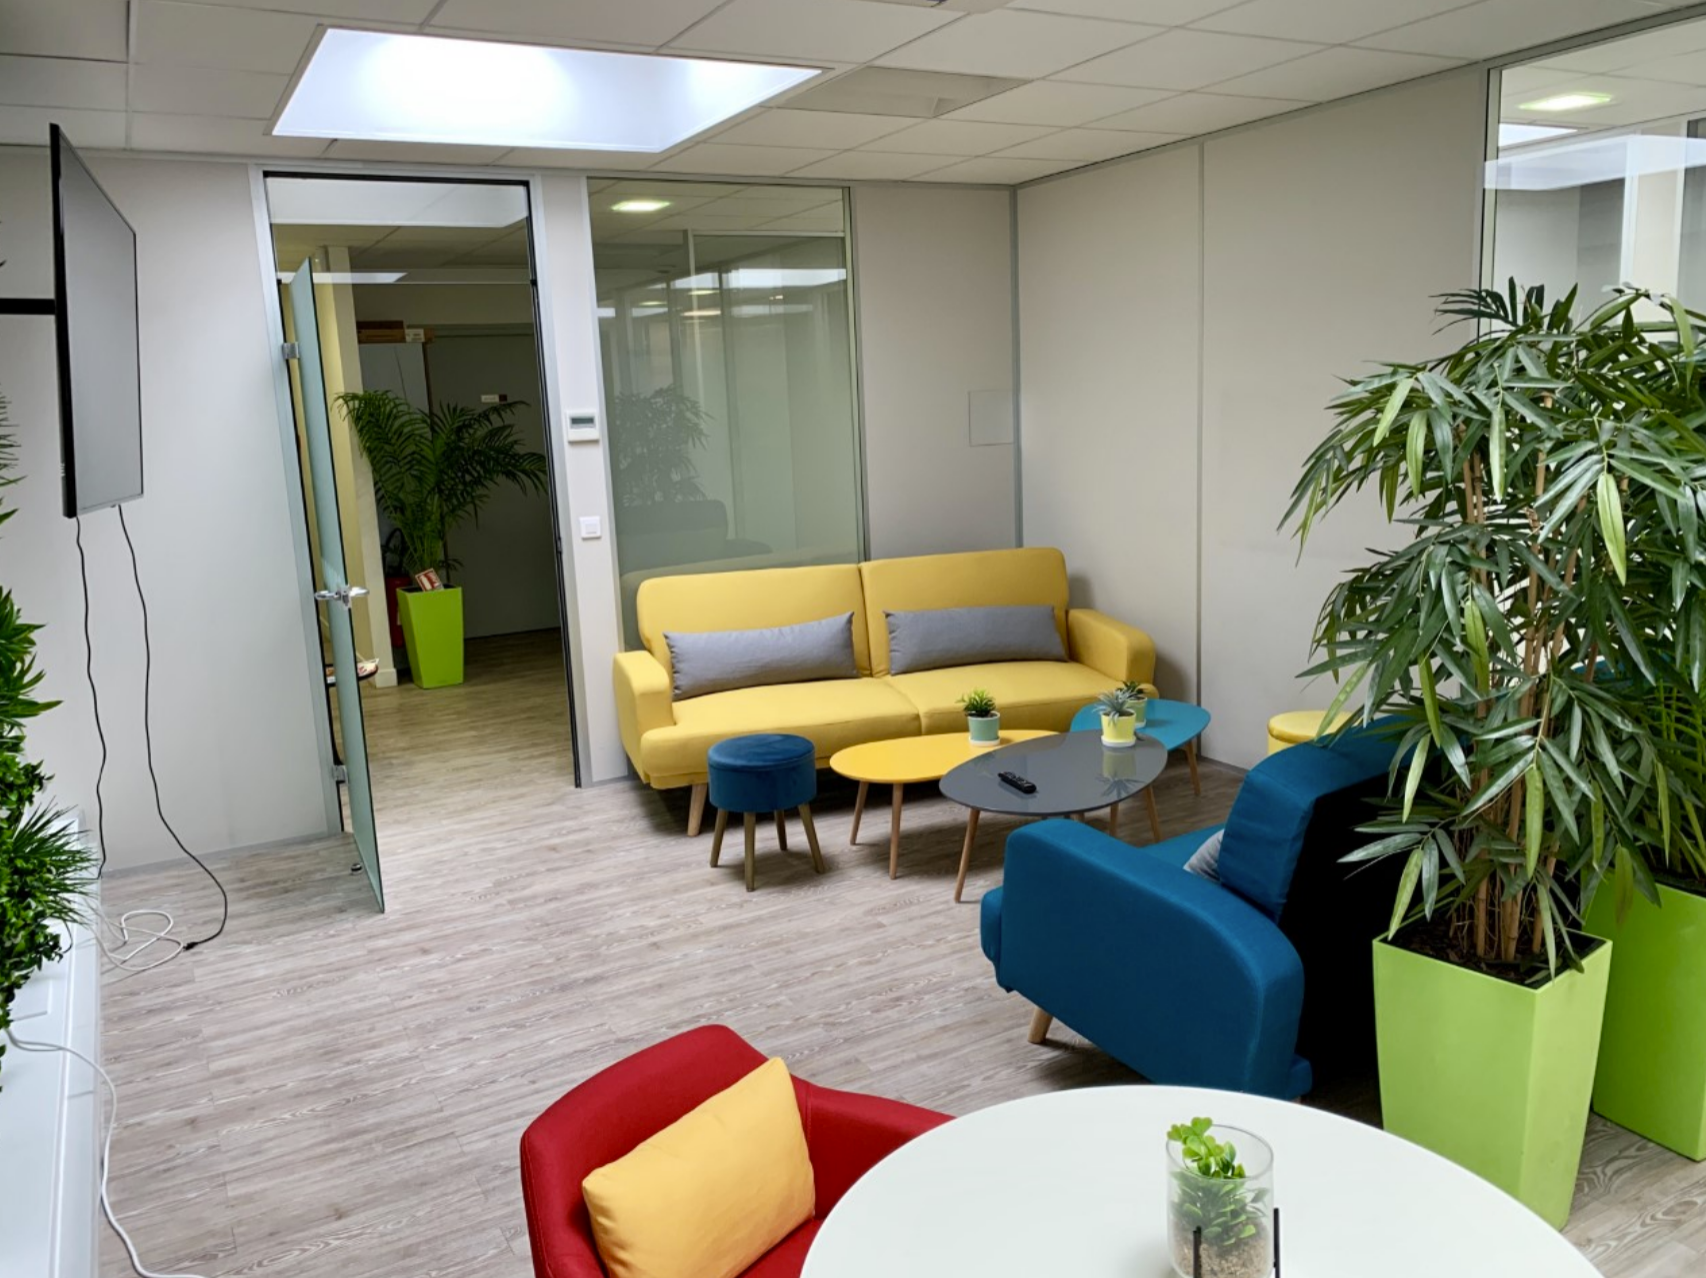
\includegraphics[width=12cm]{images/photos/bureaux_galigeo.png}
    \caption{Bureaux de Galigeo, 87 avenue d'Italie, 75013 Paris}
    \label{fig:offices}
\end{figure}


\subsection{Organisation interne}

Galigéo est composé actuellement d’une vingtaine d’employés répartis dans 5 pôles : Administratif, Commercial, Marketing, Comptabilité, Consulting et Recherche et Développement.

Le pôle administratif est le pôle qui s’occupe de la gestion du budget, du personnel et des missions à Galigeo.

Le pôle commercial gère les relations clients, il propose des offres à de nouveaux ou anciens clients, prospecte et cherche à faire grandir le cercle de clientèle de Galigeo.

Le pôle marketing imagine les produits, met en place les stratégies de pénétration du marché et réalise un catalogue de solutions que Galigeo peut fournir.

Le pôle comptabilité est responsable de la facturation des clients et la gestion interne des frais de personnels, des salaires, du matériel, etc.

Le pôle consulting est dédié à la réponse aux besoins techniques du client, il permet de rester proche du client. Il imagine les solutions retenues et les intègre dans les outils Galigeo mis à disposition pour l’entreprise.


Pour ma part, j’ai rejoint le pôle Recherche et Développement. L’équipe est composée de développeur, de testeurs, de designeurs, de data scientist, etc. Elle s’attache à améliorer les produits de Galigeo et à faire du support, de la maintenance et de l’innovation. Lorsqu’un consultant est en charge d’un projet pour un client, il s’appuie sur un ou plusieurs membres de l’équipe R\&D pour conseiller ou réaliser les tâches techniques.

\paragraph*{}

J’ai principalement travaillé avec Raimana Teina, Data Sientist chez Galigeo autour du grand projet actuel chez Galigeo « Prédiction de flux piéton » que je détaillerai dans la suite de ce rapport. Cependant j’ai également eu l’occasion de travailler sur des projets clients avec l’équipe consulting. 

% Image of the offices
\begin{figure}[H]
    \centering
    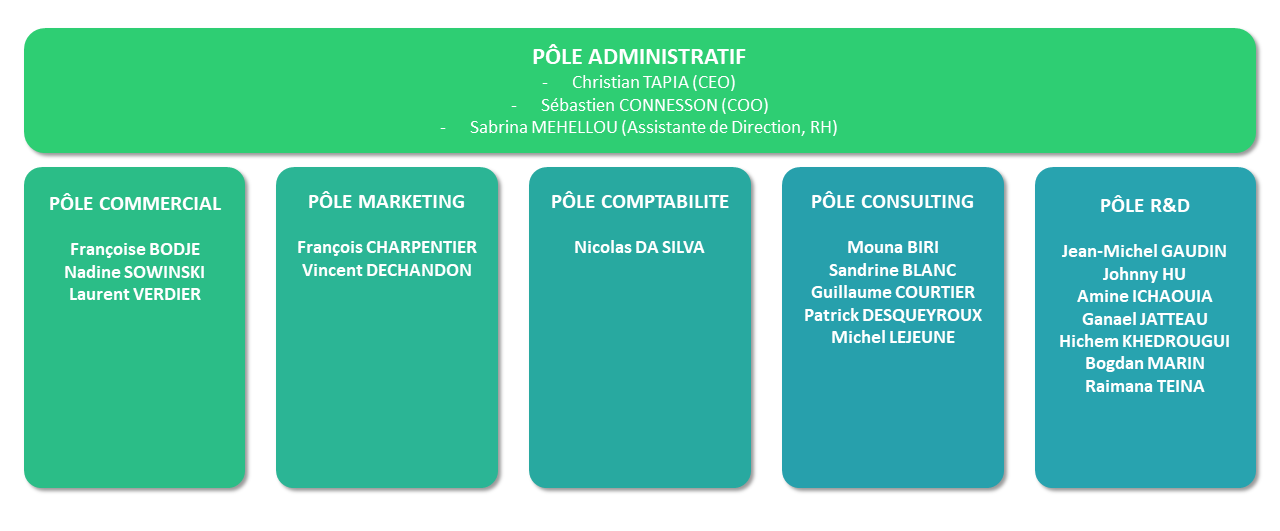
\includegraphics[width=\linewidth]{images/graphs/organigramme.png}
    \caption{Organigramme de Galigeo}
    \label{fig:organigrame}
\end{figure}


\section{Les objectifs de Galigeo}

\subsection{Les manques actuels}

Aujourd’hui, Galigeo cherche à mettre en avant des modèles prédictifs au service du géomarketing pour ses clients. Une mesure importante en géomarketing est l’estimation de flux piéton à un endroit donné et sur une période donnée. Jusqu’ici, Galigeo utilisait un service tiers afin d’obtenir une estimation de flux piéton. Cette solution de transition possède néanmoins de nombreux défauts. Tout d’abord Galigeo n’avait aucune visibilité sur les algorithmes utilisés pour faire cette estimation.

Il était alors difficile d’utiliser les résultats de cette estimation dans l’entraînement de nouveaux modèles de prédiction (estimation de chiffre d’affaires, estimation de parts de marchés, etc.). De plus, les coûts d’une telle solution restent élevés.

Il a donc été décidé de créer un modèle d’estimation de flux piéton propre à Galigeo sur lequel l’entreprise aurait accès à toutes les données d’entrées du modèle. Ainsi elle pourra modéliser d’autres variables essentielles au géomarketing plus facilement et avec une meilleure qualité. En effet, en connaissance des biais de notre modèle, ils seront plus faciles à corriger dans d’autres cas d’utilisation.

Galigeo souhaite également renforcer son équipe big data afin de mettre en valeur de grosses quantités de données brutes inexploitables en l’état. En recrutant de nouveaux data scientist, elle libèrera du temps à ses consultants et déchargera les équipes spécialisées dans la data actuellement en place.

\paragraph*{}

Après un entretien au printemps 2022 chez Galigeo et cette explication des manques et objectifs de l’entreprise à court terme, j’ai fait part de mon envie de réaliser un stage au sein de l’équipe R\&D. Ils ont retenu ma candidature et j’ai donc commencé mon stage de fin d’étude le 02 Mai 2022.


\subsection{Les objectifs du stage}

Durant ce stage j’avais donc comme première objectif de découvrir le géomarketing dans son ensemble. J’ai dû analyser et comprendre les cas d’usages métiers et me plonger dans le fonctionnement d’une équipe de développement logiciel.

J’avais également pour mission de concevoir et spécifier des solutions d’acquisition, de cleaning et de traitement des données. Comprendre le fonctionnement des produits Galigeo m’a permis de collecter et stocker la donnée de manière optimale afin de faciliter l’implémentation dans des bases de données.

J’avais également pour mission de développer des chaînes de collecte de la donnée en m’appuyant sur des méthodes de data engineering \footnote{Ingénierie des données}. Pour pouvoir par la suite utiliser au mieux la donnée dans des processus d’analyse et de traitement.

Pour la partie traitement de la donnée brute, mes objectifs étaient de développer des algorithmes et des traitements de la data grâce à des méthodes statistiques et de machine learning. Mon objectif était de transformer de la donnée brute inexploitable en une donnée pertinente pour le géomarketing des clients Galigeo.

\paragraph*{}

Mon objectif était également de m’intégrer aux équipes de Galigeo afin de mieux comprendre les objectifs de l’entreprise à long terme et les directions à prendre.


\subsection{Les objectifs à plus long terme}

Galigeo cherche aujourd’hui à implémenter de plus en plus de modèles prédictifs dans ses solutions. Pour cela, elle veut s’appuyer sur la big data et la data science qui permettent d’obtenir des résultats de qualité et qui intéressent aujourd’hui le marché du géodécisionnel.

Galigeo cherche donc à développer son équipe R\&D spécialisée dans la data afin de créer de nouveaux modèles compétitifs vis-à-vis des solutions concurrentes existantes et ainsi attirer de nouveaux clients et apporter des nouveautés aux plus anciens.

\paragraph*{}

Aujourd’hui ces modèles prédictifs permettent d’évaluer une variable à un endroit spécifique (footfall \footnote{Flux piéton}, chiffre d’affaires, cannibalisation, …). On peut alors comparer plusieurs localisations et déterminer laquelle est la plus intéressante pour une entreprise.

Il sera alors pertinent de s’intéresser à des modèles de recherche qui permettent de trouver directement la meilleure localisation pour une variable donnée.


\section{Organisation du stage}

\subsection{Planning}

Le planning complet de mon stage est disponible en annexe \ref{planning_gannt}. Il est détaillé sur la période Mai - Septembre 2022. La rédaction de ce rapport a eu lieu avant la définition des tâches d'octobre.

\subsection{Mes missions}

Ma mission principale à Galigeo était de réaliser des modèles prédictifs de variables utiles au géomarketing. L’estimation du flux piéton en une adresse a été ma principale mission. Cependant j’ai également passé quelques temps sur la modélisation de chiffres d’affaires pour une marque de produit culturel et électronique française. J’ai dû également modéliser la cannibalisation qu’entraînerait l’ouverture d’une enseigne proche d’une autre sur le territoire français.

\paragraph*{}

Ces deux missions mettaient en pratique mes compétences en Machine Learning acquises à l’ENSG. Je reviendrai sur ma mission sur le flux piéton dans la partie 2.2 de ce rapport. Pour la partie modélisation de chiffres d’affaires et d’estimation de cannibalisation, j’y reviendrai dans la partie 2.3.

\paragraph*{}

J’ai également réalisé d’autres plus petites missions pour Galigeo. J’ai eu la chance de travailler quelques jours sur un projet d’analyse de données et sur un projet de data engineering pour une compagnie internationale. Je détaillerai rapidement ces deux derniers projets dans la partie 2.4 de mon rapport.


\subsection{Relations internes et client}

Dans le pôle R\&D, le travail est organisé autour de la méthode Agile \footnote{Méthode de travail en équipe}. Un sprint \footnote{Rassemblement de tâches à executer dans un temps donné} dure environ 2 semaines et nous faisons un point tous les jours à 15h30 pour communiquer sur notre avancement et les difficultés rencontrés afin de pouvoir répondre rapidement aux besoins de chacun.

Je peux télétravailler 2 jours par semaine et cela fonctionne très bien car la plupart des réunions en présentiel sont également retransmises en visio-conférence. Galigeo utilise la suite Office 365 Professionnel ce qui permet d’organiser facilement le travail et les interactions.

\paragraph*{}

J’ai également travaillé sur des projets où j’échangeais uniquement avec le pôle consulting. Dans ce cas-là, nous avions des réunions quotidiennes également avec le consultant en question et une réunion hebdomadaire avec le client.

\chapter[Le stage \ensg]{Le stage}

\section{Généralités}

Dans la suite de ce rapport je vais me consacrer sur les deux missions principales que j’ai réalisées à Galigeo. La première est l’estimation d’un flux piéton à une adresse donnée. (2.2) Ce n’est pas une mission réalisée pour un client en particulier, c’est une fonctionnalité qui a été ajoutée dans la dernière version des logiciels SaS de Galigeo et est donc accessible pour tous les utilisateurs du service.

\paragraph*{}

La deuxième mission est une demande spécifique d’un client de Galigeo. J’ai eu accès à des données confidentielles à l’entreprise. Toutes les illustrations, schémas ou fragments de données, pour cette partie, seront donc fictifs

\paragraph*{}

Enfin, je terminerai rapidement sur deux autres missions clients, plus secondaires pour lesquels je rentrerai moins dans le détail.


\section{Prédiction de flux piéton}

\subsection{Mise en contexte}

Le flux piéton est une très bonne variable pour estimer le flux de consommateurs potentiels qui passe chaque jour devant une enseigne commerciale. Il est donc essentiel pour une entreprise qui fournit des services de géomarketing, de pouvoir estimer au mieux cette variable.

\paragraph*{}

Jusqu’aujourd’hui, Galigeo s’appuyait sur des estimations calculées par une autre entreprise ce qui l’empêchait de corriger les biais et erreurs possibles. Elle n’avait pas la main sur les algorithmes d’estimations.

\paragraph*{}

Ma mission a donc été de réaliser cet algorithme d’estimation du flux moyen de piéton sur une année autour d’une adresse donnée et ce pour l'ensemble du territoire national.

\paragraph{}

Il a fallu néanmoins prendre en compte les contraintes techniques de l’entreprise, les biais qui pouvaient être présents dans la donnée utilisée et l’efficacité de l’algorithme. Si les temps de calculs sont trop longs, l’expérience utilisateur risque d’être impactée mais il faut garder un modèle puissant afin de minimiser les erreurs de prédiction.

\subsection{La donnée}

Pour estimer ce flux piéton, nous allons nous appuyer sur des mesures quotidiennes que Galigeo achète à un fournisseur. En effet, Galigeo reçoit quotidiennement des positions de cellulaires sur l'ensemble du territoire métropolitain. Elle en reçoit environ 70M par mois, chacune correspondant à un évènement de visite. Cette donnée est collectée via des applications mobiles qui sont autorisées à transmettre la position du smartphone au fournisseur de Galigéo. Les positions sont anonymes mais possèdent un identifiant de smartphone ce qui permet d'avoir aussi des informations de déplacements. La donnée brute est structurée comme ci-dessous :

\begin{table}[H]
    \centering
    \begin{tabular}{|l|l|}
    \hline
    \textbf{Attribut} & \textbf{Description}              \\ \hline
    idEvent           & Id de l'évènement                 \\ \hline
    uuid              & Id du smartphone                  \\ \hline
    latitude          & Latitude de l'évènement           \\ \hline
    longitude         & Longitude de l'évènement          \\ \hline
    accuracy          & Précision de la localisation      \\ \hline
    arrival           & Date d'arrivée à la localisation  \\ \hline
    departure         & Date de départ de la localisation \\ \hline
    \end{tabular}
    \caption{Résumé de la structure d'un évènement de visite}
\end{table}

\paragraph*{}

Nous avons également utilisé de la donnée économique pour enrichir notre modèle. En effet Open Street Map propose une base open-source de POI structurée comme ci-dessous :

\begin{table}[H]
    \centering
    \begin{tabular}{|l|l|}
    \hline
    \textbf{Attribut} & \textbf{Description}                                  \\ \hline
    id\_poi           & Id du poi                                             \\ \hline
    type              & Nature du POI (Magasins, Restaurants, Epiceries, ...) \\ \hline
    latitude          & Latitude du POI                                       \\ \hline
    longitude         & Longitude du POI                                      \\ \hline
    \end{tabular}
    \caption{Structure d'un POI}
\end{table}

\paragraph*{}

Il était également intéressant de rajouter de la donnée démographique à notre modèle. Pour cela nous avons utilisé les données de population de l'INSEE agrégées au niveau des IRIS géographiques.

\paragraph*{}

Nous allons utiliser des algorithmes de Machine Learning pour estimer ce trafic piéton. Il nous faut donc des données mesurées sur le terrain afin d'entraîner un modèle. Galigeo possède plus de 11000 mesures réparties plus ou moins équitablement sur le territoire même si la plupart d'entre elles sont en milieu urbain.

\begin{figure}[H]
    \centering
    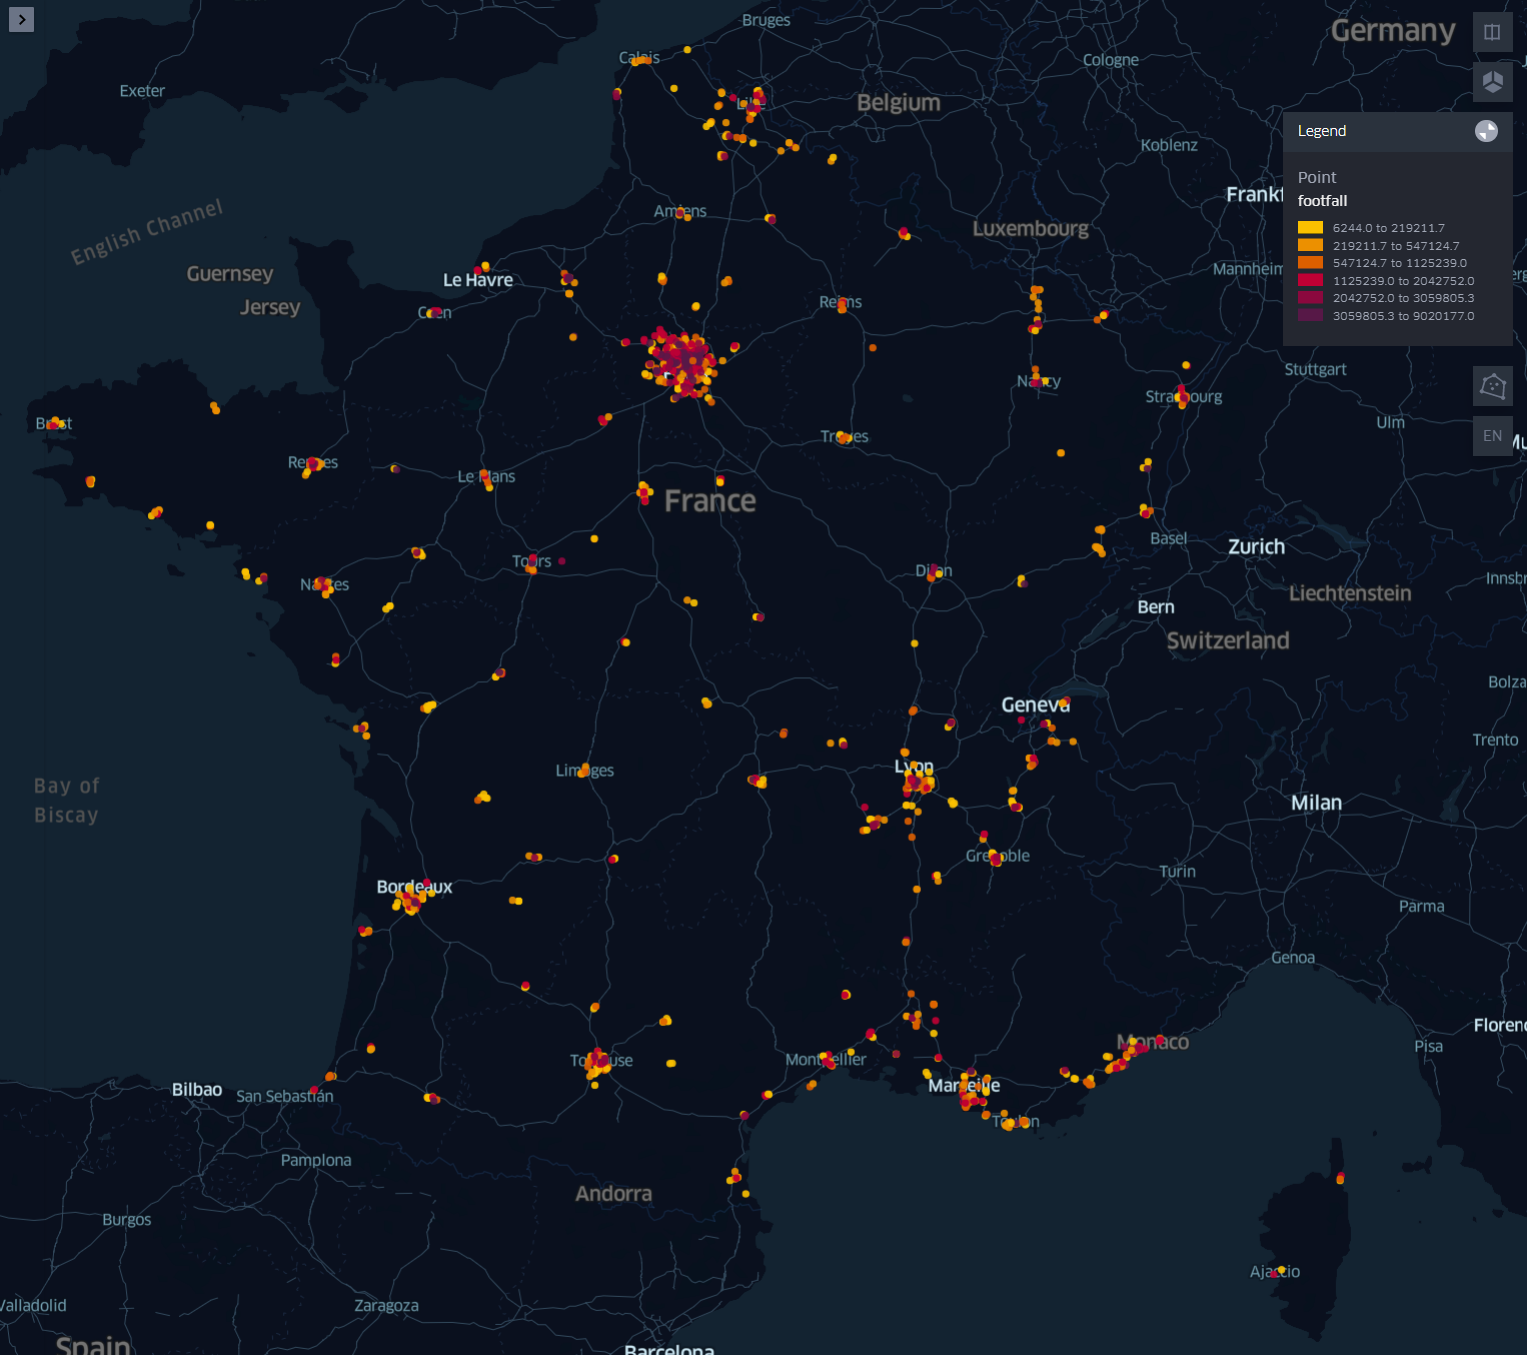
\includegraphics[width=\linewidth]{images/graphs/map_of_label_footfall.png}
    \caption{Carte des données d'entraînement}
    \label{fig:footfallmap}
\end{figure}

\subsection{Technologies utilisées}

\subsubsection{Agrégation spatiale}

Une fois que nous avons l'ensemble de nos données nous remarquons qu'elles se distinguent en deux groupes de par leur nature. Les données ponctuelles (\'Evènements de visites, POI, etc.) et les données surfaciques (Population par IRIS). Pour homogénéiser notre donnée et simplifier les futurs calculs il est important de segmenter l'espace et ajouter un index spatial à nos données.

Nous nous sommes dirigés vers la solution des hexagones H3 \cite{Uber_H3} développés par Uber. C'est un système d'indexation géospatiale qui constitue un pavage hexagonal de la sphère multi-échelles et dont les index sont hiérarchiques.

Dans notre cas c'est la solution optimale car nous pouvons l'utiliser pour joindre nos données disparates, le format hexagonal facilite la modélisation des flux et est bien adapté pour appliquer le machine learning aux données géospatiales.


% Image of the offices
\begin{figure}[H]
    \centering
    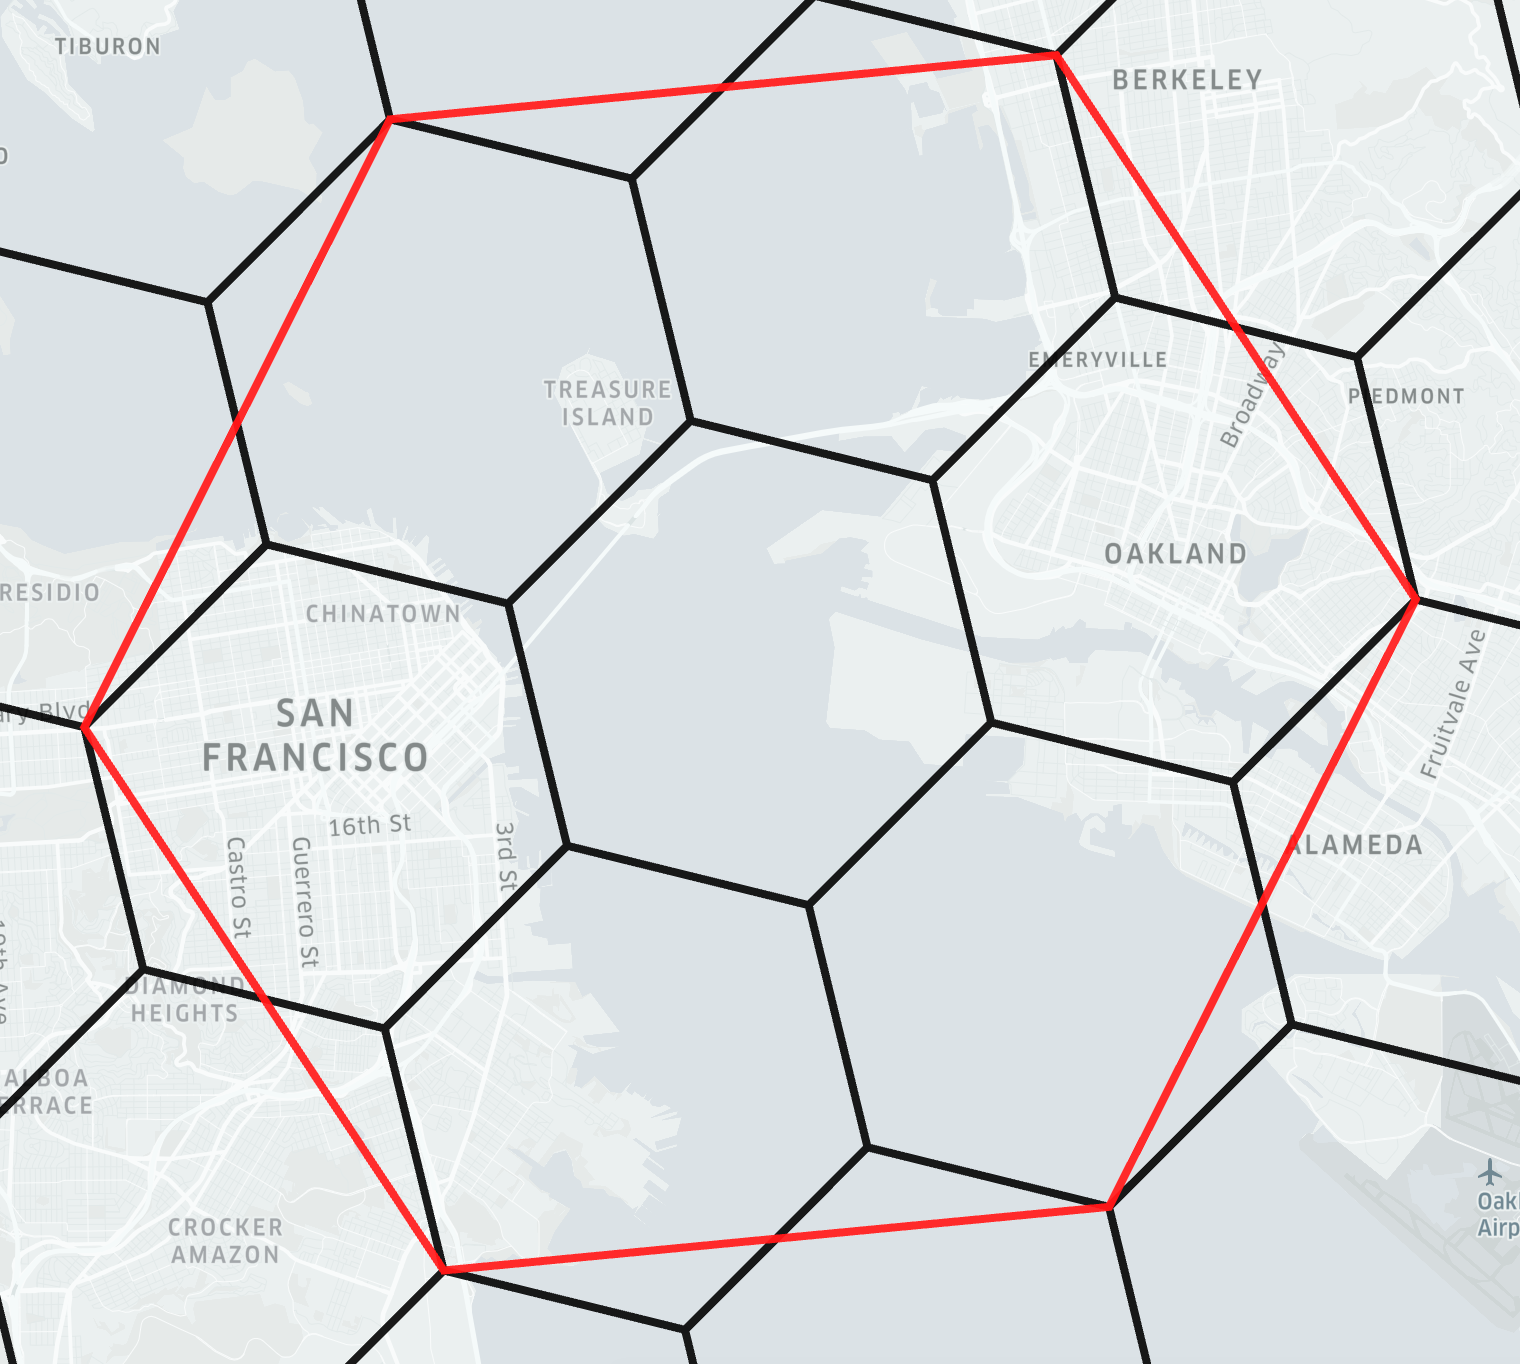
\includegraphics[width=7cm]{images/graphs/h3-multiscale.png}
    \caption{Principe de multi-echelles des cellules H3}
    \label{fig:celluleh3}
\end{figure}

\begin{figure}[H]
    \centering
    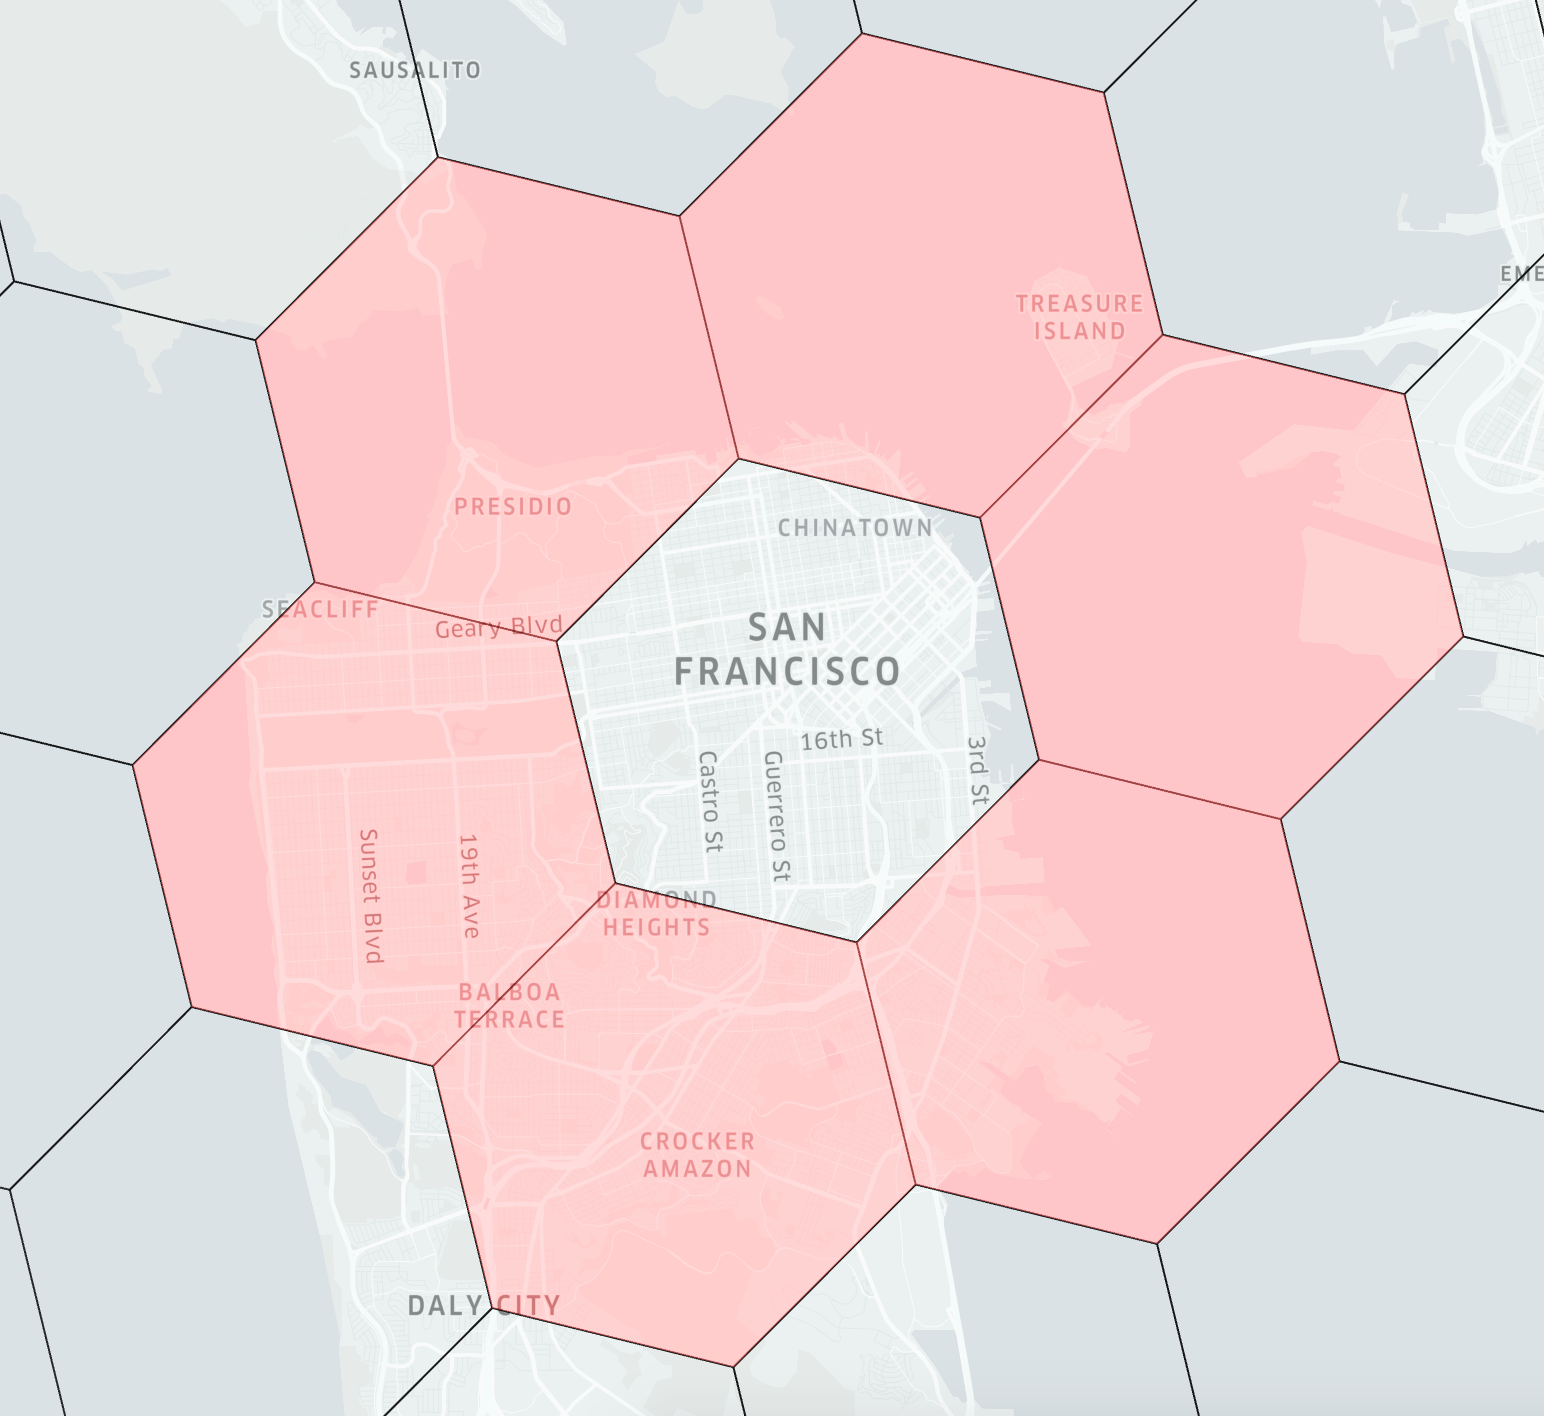
\includegraphics[width=7cm]{images/graphs/h3-ring.png}
    \captionsetup{justification=centering}
    \caption{Les 6 voisins d'une cellule H3 se rapproche d'un cercle, utile pour la modélisation de flux}
    \label{fig:celluleh3ring}
\end{figure}

Pour notre part on choisira le niveau d'échelle 11, ce qui correspond environ à un hexagone de 27 mètres de rayon.

\subsubsection{Infrastructure de base de données}

Pour stocker toutes ces données, Galigeo utilise un service de Cloud Computing \footnote{Ensemble de services et de machines informatiques délocalisés dans un cloud} nommé Google Cloud Plateform (GCP) qui permet de stocker une grande quantité de données et de faire des calculs plus ou moins complexes sur celle-ci.

\paragraph*{}

Un des grands avantages de cette solution est l'intégration de Tensorflow, une bibliothèque open-source développée par Google pour faire du machine learning et de l'intelligence artificielle. Elle est très utile pour l'entraînement de réseaux de neurones profonds (DNN).

Nous pouvons également y combiner Keras, une interface open-source conçue pour simplifier l'utilisation de Tensorflow.


\subsubsection{Type de modèle utilisé}

\'Etant donnés les choix précédents, nous nous sommes donc orientés vers un modèle de Deep Neural Network (DNN).

Il est cependant important de noter que les modèles de Deep Neural Network, prouvent leur meilleure efficacité par rapport à d'autre modèles de Machine Learning lorsque la donnée est non structurée et que la taille du dataset \footnote{Tableau de données} est importante (plusieurs millions de lignes)

Dans notre cas, ces conditions ne sont pas remplies mais nous verrons plus tard dans ce rapport les alternatives envisagées.


\subsection{Préparation des données}

\subsubsection{Structuration des données}

Cette étape est cruciale pour obtenir des bons résultats après la modélisation. Il s'agit de passer de la donnée brute présentée précédemment à une donnée structurée qui permettra d'entraîner le réseau de neurones.

Pour cela, nous avons projeté l'ensemble de notre donnée brute sur la grille H3 d'Uber. Pour chaque valeur de flux piéton mesuré, nous avons calculé le nombre de visites dans la même cellule ainsi que dans les cellules voisines. Nous avons agrégé ces données events par mois sur une année complète de septembre 2021 à août 2022.

Nous avons appliqué le même principe spatial pour les POIs. Les cellules voisines se calculent très facilement grâce aux fonctions open-source mises à disposition. Ainsi on peut calculer différents anneaux autour de notre cellule de départ.


\begin{figure}[H]
    \centering
    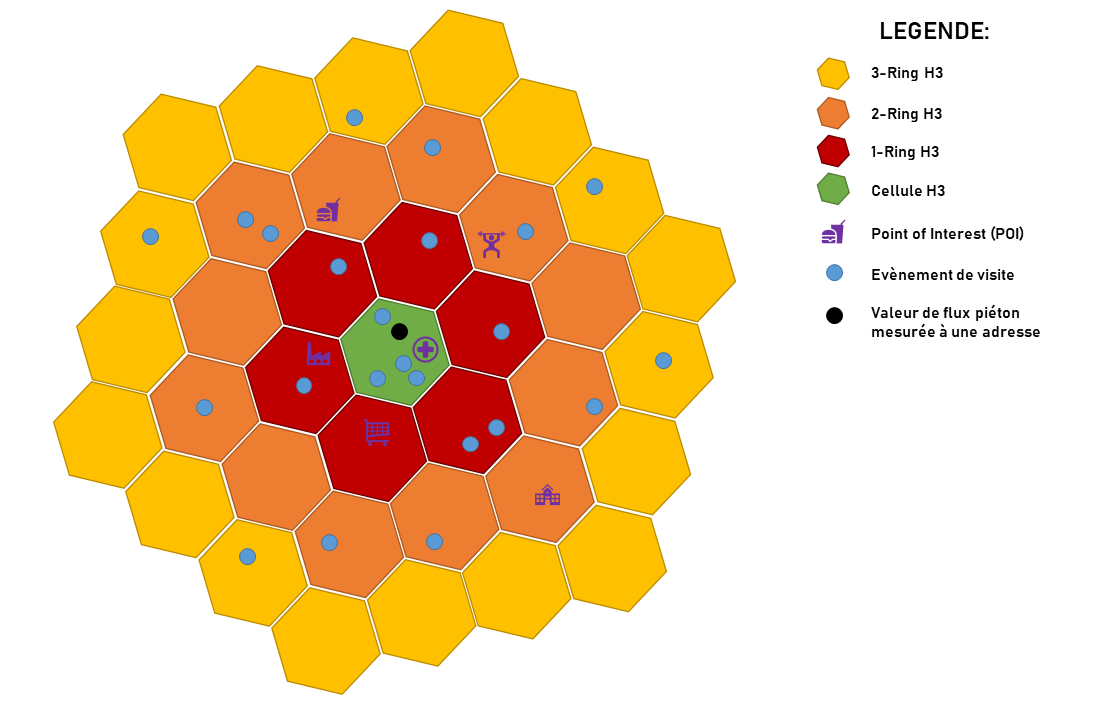
\includegraphics[width=\linewidth]{images/graphs/dataset.png}
    \captionsetup{justification=centering}
    \caption{Agrégation des données aux cellules H3 pour générer un dataset}
    \label{fig:dataset_aggregation}
\end{figure}

Pour ce qui est de la donnée de population, nous avons simplement pris le centroïde de la cellule H3, et l'avons intersecté avec les géométries des IRIS françaises afin de déterminer dans quel IRIS la cellule se trouve.

Nous avons obtenu alors une structure de dataset comme ci-dessous. Une feature est un paramètre du modèle et le label est la variable à estimer.


\begin{table}[H]
    \centering
    \begin{tabular}{|l|l|l|}
    \hline
    \textbf{Colonnes}    & \textbf{Type} & \textbf{Description}                                                    \\ \hline
    h3\_index            &               & Index de la cellule H3                                                  \\ \hline
    visits\_MMAAAA & feature       & Nb events dans la cellule H3 par mois (x12)                        \\ \hline
    visits        & feature       & Nb events dans la cellule H3 sur l'année                          \\ \hline
    visits\_k1     & feature       & Nb events dans la cellule H3 et l'anneau 1 sur l'année            \\ \hline
    visits\_k2     & feature       & Nb events dans la cellule H3 et les anneaux 1, 2 sur l'année       \\ \hline
    visits\_k3     & feature       & Nb events dans la cellule H3 et les anneaux 1, 2, 3 sur l'année    \\ \hline
    visits\_k4     & feature       & Nb events dans la cellule H3 et les anneaux 1, 2, 3, 4 sur l'année \\ \hline
    poi\_N        & feature       & Nb de POI dans la cellule H3 par nature                                 \\ \hline
    poi\_N\_k1    & feature       & Nb de POI dans la cellule H3 et l'anneau 1 par nature                   \\ \hline
    poi\_N\_k2    & feature       & Nb de POI dans la cellule H3 et les anneaux 1, 2 par nature              \\ \hline
    poi\_N\_k3    & feature       & Nb de POI dans la cellule H3 et les anneaux 1, 2, 3 par nature           \\ \hline
    poi\_N\_k4    & feature       & Nb de POI dans la cellule H3 et les anneaux 1, 2 , 3 , 4 par nature      \\ \hline
    population           & feature       & Population in the IRIS of the H3 cell                                   \\ \hline
    footfall             & label         & Flux piéton mesuré en un point de la cellule H3                         \\ \hline
    \end{tabular}
    \caption{Structure du dataset}
    \end{table}

On obtient alors un dataset d'environ 11000 lignes et 14 colonnes.

\subsubsection{Nettoyage des données}

La deuxième étape de la préparation des données consiste à les nettoyer pour supprimer d'abord les lignes où il manquerait certaines variables puis celles dont les valeurs du label sont aberrantes.

On se retrouve alors avec un dataset réduit de 40\%, il reste environ 6500 lignes.

\paragraph{}


Une fois ces deux étapes réalisées, nous pouvons sortir différents graphiques statistiques disponibles en annexe : KDE, Matrice de corrélation, Répartition des features.


\subsection{Tuner et Entraînement du modèle}

Notre dataset est maintenant prêt à être utilisé comme base d'apprentissage. Nous avons donc créé une structure de modèle. Cette structure possède des paramètres appelés Hyperparamètres. Chaque hyperparamètre peut prendre une valeur parmi une liste bien définie. Le principe du Tuner est de compiler ce modèle plusieurs fois avec des valeurs d'hyperparamètre bien différentes et choisies aléatoirement.

\begin{figure}[H]
    \centering
    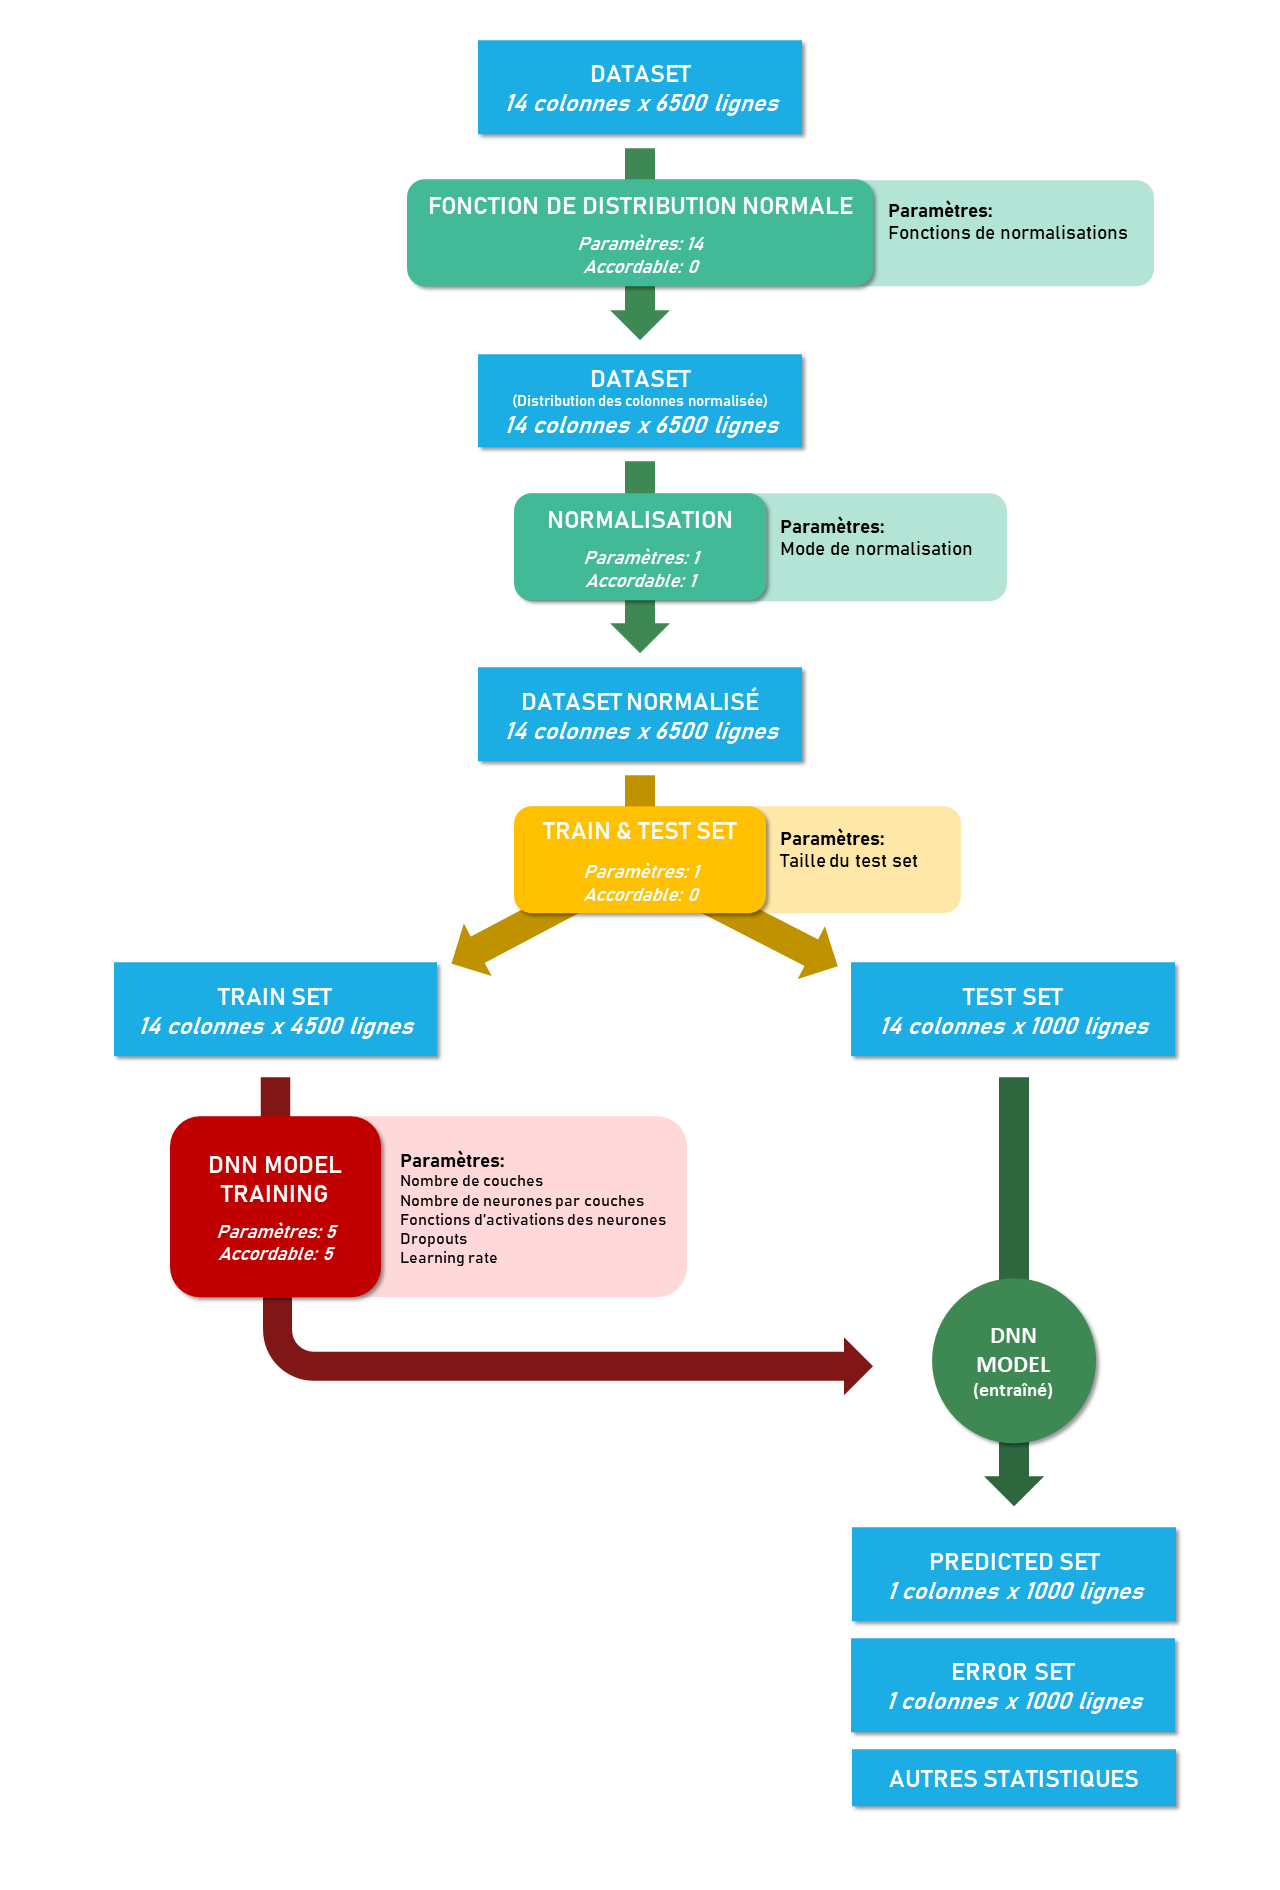
\includegraphics[width=\linewidth]{images/graphs/struc_model_dnn.png}
    \captionsetup{justification=centering}
    \caption{Structure du modèle envisagé}
    \label{fig:strcu_dnn}
\end{figure}

La première étape de notre modèle est donc de normaliser la distribution de nos features. En effet, la distribution des valeurs pour chaque features n'est pas forcément "normale" et il est préférable de passer nos valeurs à travers une fonction pour la modifier.

\begin{figure}[H]
    \centering
    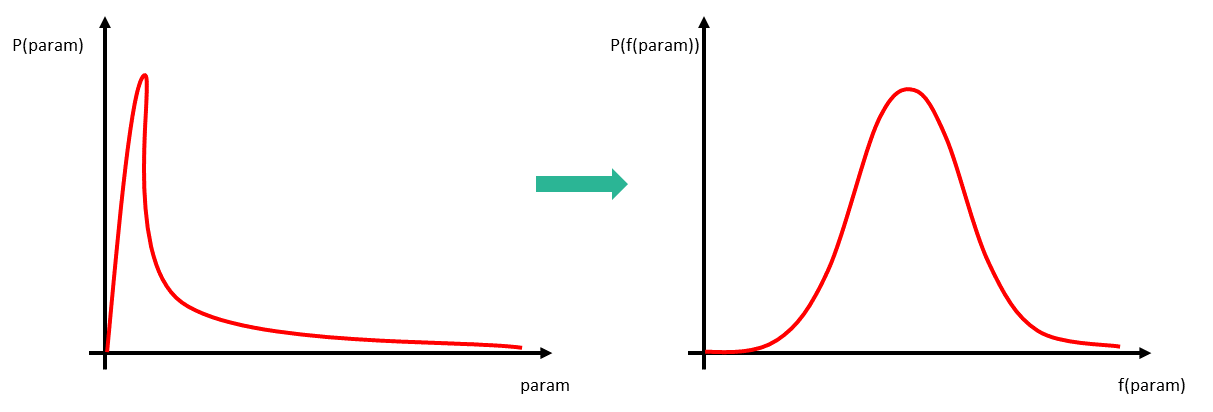
\includegraphics[width=\linewidth]{images/graphs/fct_histo.png}
    \captionsetup{justification=centering}
    \caption{Principe de normalisation de la distribution d'une feature}
    \label{fig:fct_repartition}
\end{figure}

L'étape suivante est de normaliser les valeurs de nos features (cette fois ci, on ne modifie pas le label). Pour cela, il existe principalement deux types de normalisation : La normalisation min/max et la normalisation moyenne/écart-type.

Cela permet entre autre d'assurer une cohérence entre les données et permet à l'exécution d'être plus rapide et meilleure.


\paragraph{}

Une fois cette étape réalisée, nous divisons en deux parties aléatoires (la proportion est contrôlée) le dataset normalisé. La partie "trainset" permet d'entraîner le modèle et la partie "testset" permet de vérifier si le modèle est correctement entraîné.

\paragraph{}

L'objectif est maintenant d'obtenir un réseau de neurones entraîné. Pour cela, nous utilisons un modèle construit sur les hyperparamètres et lui passons l'ensemble du trainset en entrée. En parcourant l'ensemble des données et en essayant d'estimer le label, le réseau de neurone apprend et règle ses paramètres internes (poids des axones, valeur interne des neurones, etc.) en appliquant une validation croisée.

De cette étape, nous récupérons un réseau de neurones profonds qui permet maintenant d'estimer notre label en fonction de nos features.


\paragraph{}

Nous passons donc notre testset dans notre réseau neuronal. Cela nous permet d'obtenir notre label estimé et de le comparer au vrai label. On obtient alors une liste de n erreurs (dans notre cas 1000), grâce auxquels nous pouvons mesurer la qualité du réseau de neurones. On peut calculer l'erreur quadratique moyenne (RMSE), un coefficient de détermination (R2) ou la précision du modèle ("accuracy").

\subsection{Résultats}

\begin{table}[H]
    \centering
    \begin{tabular}{l|l|l|}
    \cline{2-3}
                                            & \textbf{Test set} & \textbf{Training set} \\ \hline
    \multicolumn{1}{|l|}{\textbf{RMSE}}     & 1 000 000         & 500 000                \\ \hline
    \multicolumn{1}{|l|}{\textbf{R2 Score}} & 0.45              & 0.86                  \\ \hline
    \end{tabular}
    \caption{Résumé des résultats}
\end{table}

Pour estimer la qualité de notre modèle, il faut regarder les résultats de la colonne de gauche, "Test set". On remarque tout de suite que l’erreur moyenne quadratique est d’environ 1000000. Or, si l’on se réfère à l’annexe B, Statistiques du modèle, on remarque que le flux piéton médian est de 1000000 également.

Le R2 score est également faible. Idéalement, il devrait se rapprocher de 1. L’estimation que fait le modèle n’est donc pas encore suffisante. 

\paragraph*{}

Cependant Galigeo renforce son dataset à chaque arrivée de données ce qui peut améliorer les résultats par la suite. Il se peut également que 6500 entrées soit trop peu et que l’enrichissement de mesure permette également de rendre plus précises les estimations du modèle.

Nous avons également discuté de nombreuses autres pistes pour obtenir des résultats plus intéressant mais je les détaillerai dans la partie 3.1 de ce rapport.

\section{Prédiction de chiffre d'affaire}

\subsection{Contexte}

Pour qu’une entreprise continue à croître et à se développer, elle peut étendre son aire d’attraction et ainsi cibler plus de clients. L’entreprise décide alors d’ouvrir une nouvelle enseigne. Le choix de l’emplacement est alors stratégique.

Pour ce projet, un client de Galigeo souhaite implanter de nouvelles enseignes sur le territoire français. Pour ce faire il souhaite estimer le chiffre d’affaires qu’engendrerait un magasin en fonction de sa localisation, de sa surface, du type de magasin et du flux piéton moyen à l’adresse. 

\paragraph{}

Il a donc fallu créer un modèle prédictif du chiffre d’affaires en s’entraînant sur les données des enseignes existantes. Cependant, cette entreprise possède 150 enseignes environ en France et cela semble insuffisant pour entraîner un modèle de machine learning. Nous avons donc utilisé une autre méthode pour démultiplier les données.


\subsection{Données}

La France est découpée en 15 500 IRIS (îlots Regroupés pour l'Information Statistique) et le client possède des données commerciales pour certains d’entre eux. Il est alors intéressant de travailler sur les IRIS et non sur les enseignes. En effet, nous avons à disposition :

\begin{itemize}
    \item La liste des enseignes (surface, chiffre d’affaires, type, localisation, …)
    \item La liste des concurrents (surface, type, localisation, …)
    \item Des données socio-démographiques pour chaque IRIS (tranche d’âge, nombre de ménage, revenue moyen, …)
    \item Un distancier des Iris (permet de connaitre la distance et le temps de parcours entre deux centroïdes d’Iris)
    \item Une estimation de la valeur du marché dans chaque IRIS
    \item Une valeur de chiffre d’affaires pour chaque enseigne dans chaque IRIS (C’est ici le chiffre d’affaires tracé, une partie du chiffre d’affaires de chaque enseigne ne peut pas être localisée)
\end{itemize}

\paragraph{}

On peut alors créer un dataset où chaque élément correspond à un iris pour un magasin et agréger le reste de la donnée à cette structure. On cherchera alors à estimer une part de marché, qui correspond à la quantité de marché détenu par un magasin particulier. Chaque enseigne connait l'origine géographique d'une partie de son chiffre d'affaire (~20\%), on peut donc connaitre cette part de marché sous-évaluée, en divisant ce chiffre d'affaire tracé par la valeur du marché dans un IRIS donnée.

\begin{figure}[H]
    \centering
    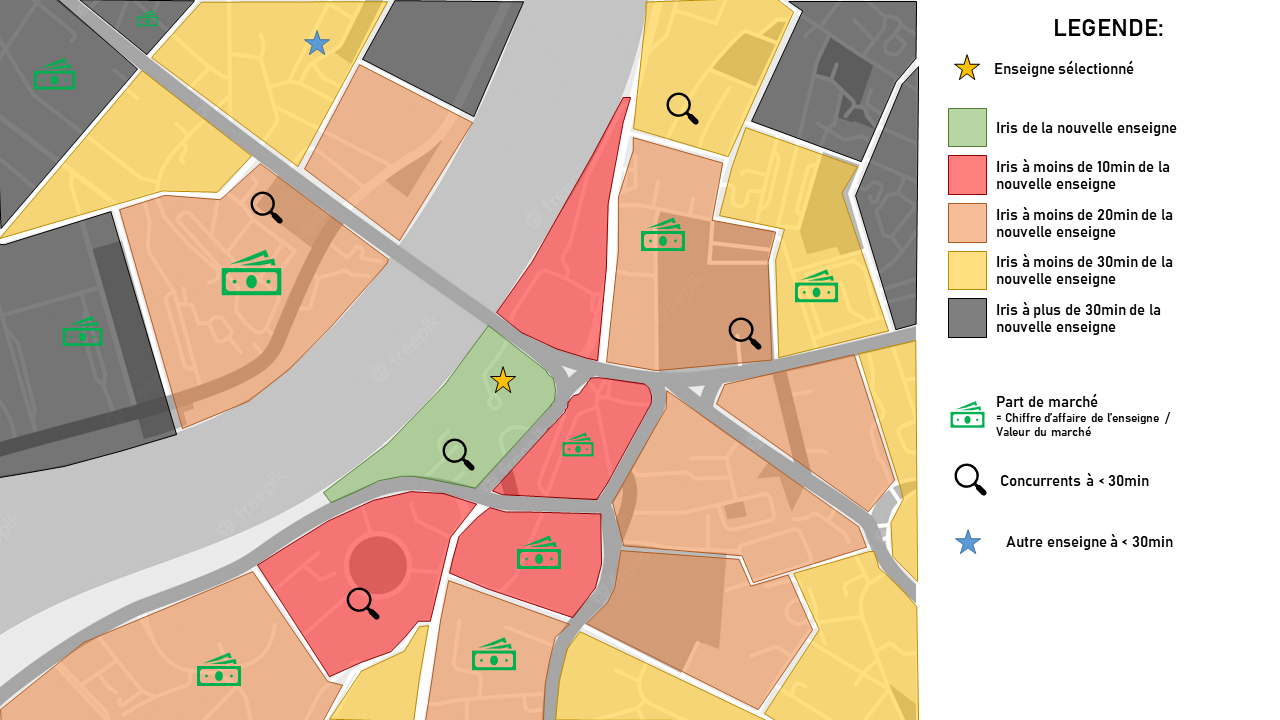
\includegraphics[width=\linewidth]{images/graphs/data_ca.png}
    \captionsetup{justification=centering}
    \caption{Résumé de l'agrégation des données}
    \label{fig:data_ca}
\end{figure}

\subsection{Structure du modèle}

Cette fois-ci, il était plus intéressant de ne pas choisir un algorithme de Deep Learning mais un algorithme de machine learning moins coûteux en ressource comme un régresseur « Random Forest » ou un « XGBoost ».
On utilisera la même structure de modèle qu’à la partie 2.2 mais cette fois-ci la normalisation est moins importante car le modèle n’est pas composé de neurones mais d’arbres de décisions.
Nous avons donc,cette fois-ci, fait deux fois la manipulation: une fois avec un régresseur XGBoost et une fois avec  un régresseur RandomForest pour choisir le modèle le mieux approprié.


\subsection{Résultats}

Grâce à nos deux modèles, nous avons pu faire des prédictions et les comparer:


\begin{figure}[H]
    \centering
    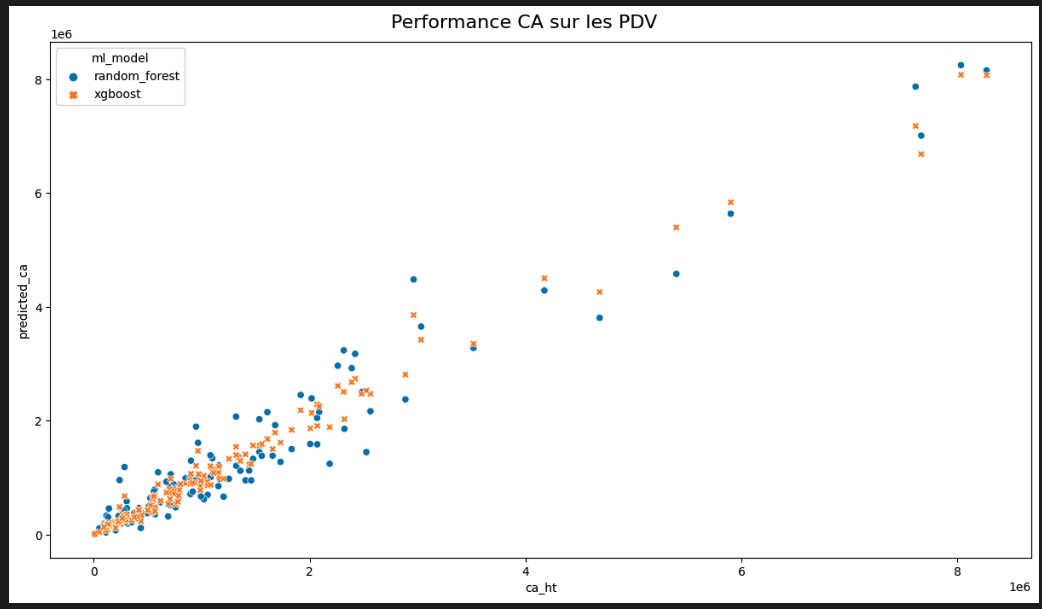
\includegraphics[width=13cm]{images/graphs/result_ca.png}
    \captionsetup{justification=centering}
    \caption{Résultat: Prédiction en fonction des mesures}
    \label{fig:result_ca}
\end{figure}

Nous avons donc choisi d'utiliser le modèle XGBoost qui nous permet d'avoir des prédiction beaucoup plus fiable.

\'A l'heure actuelle, nous attendons une réunion avec le client afin de vérifier que nos résultats concordent avec les leurs.

\section{Autres missions}

\subsection{Analyse de données - Base de données nationale des Bâtiments}

Pendant mon stage, j’ai également pu travailler sur d’autres petites missions pour des clients de Galigeo pour lesquels il n’était pas forcément question de machine learning.

\paragraph{}

Un client de Galigeo réalise de la prospection chez des particuliers. Jusqu’ici, la prospection était organisée très simplement, un quartier était sélectionné et les prospecteurs passaient dans chaque habitation. Ce client cible les habitations se chauffant à l’électricité et il arrive souvent que certaines des habitations prospectées se chauffent au gaz ou autre. Dans un souci d’économie et de gain de temps, nous avons donc tenté de cibler les prospections.

En janvier 2022, une Base de Données Nationale des Bâtiments \cite{BDNB} est mise en ligne en open-source. C’est une base très complète avec plus de 90\% des géométries renseignés. Environ 25\% des bâtiments possèdent des informations énergétiques dont on ne connait pas la qualité. Le client et Galigeo ont donc décidé de mener une campagne de prospections cet été en s’appuyant sur cette base de données afin de qualifier les données énergétiques disponibles. Nous avons donc fait de l’analyse de données sur quelques IRIS (à Rennes et à Paris) pour lancer la campagne de prospection.

\paragraph{}

Aujourd’hui les campagnes de prospections sont toujours en cours mais le résultat semble positif. Si la base de données est retenue pour diriger les campagnes de prospections du client, il faudra automatiser les processus d’analyse pour envoyer la donnée traitée dans leur application métier développée par Galigeo.

Sachant que seulement 25\% des bâtiments ont des données énergétiques, il sera peut-être intéressant un jour d’utiliser un algorithme de classification par machine learning pour interpoler ces informations manquantes sur le reste de la base. 


\subsection{Data engineering - Scrapping et automatisation de chaîne d'acquisition de données}

Une autre mission que j’ai pu réaliser était pour un client international de Galigeo. Ils utilisaient la solution de Galigeo pour leurs compagnies en France et souhaitent l’utiliser dans 13 nouveaux pays. La solution actuelle permet de sortir des rapports de géomarketing poussés qui s’appuient sur de très grandes quantités de données.

L’objectif était donc de récupérer de la donnée en quantité et d’automatiser son processus de publication dans une base de données. J’ai donc écrit des scripts permettant de scrapper des sites web de concurrents pour récupérer de la donnée non structurée pour l’organiser. J’ai aussi dû automatiser des requêtes via des API afin de récupérer des données ponctuelles sur un pays entier.

\paragraph*{}

Ce projet est encore en cours à la date où je rédige ce rapport. L’application et la base de données complète devrait être livrée pour la mi-octobre.

\evenchapter[Bilan \ensg]{Bilan}

\section{...}


%\begin{comment}
%-------------------------------------------------------------------------------
% \newevenpage
\chapter*{Conclusion}
  \addcontentsline{toc}{part}{Conclusion}
  \vspace{1.5cm}
Il est l'heure de conclure : bonne nuit !


%-------------------------------------------------------------------------------
% Insertion de la bibliographie
\newevenpage
%\printbibheading
\printbibliography[title={Bibliographie}]
\nocite{*}

\newevenpage
\listoffigures

\newevenpage
\listoftables
%----------------------------------------------------

\newevenpage
\begin{appendices} 
\label{beginappendices}
\annexe[Filtre de Kalman]{Filtre\newline de Kalman}
\label{annexekalman}
Contenu de l'annexe sur Kalman...

\annexe[Moindres carrés]{Moindres carrés}
\label{annexemc}
Contenu de l'annexe sur MC...

\end{appendices} 
%\end{comment}
\end{document}